\begin{frame}{A New Game with an Old Soul}
    \begin{minipage}{\textwidth}
        \centering
        \begin{minipage}{.495\textwidth}
            \onslide<1-2>{
                \begin{figure}
                    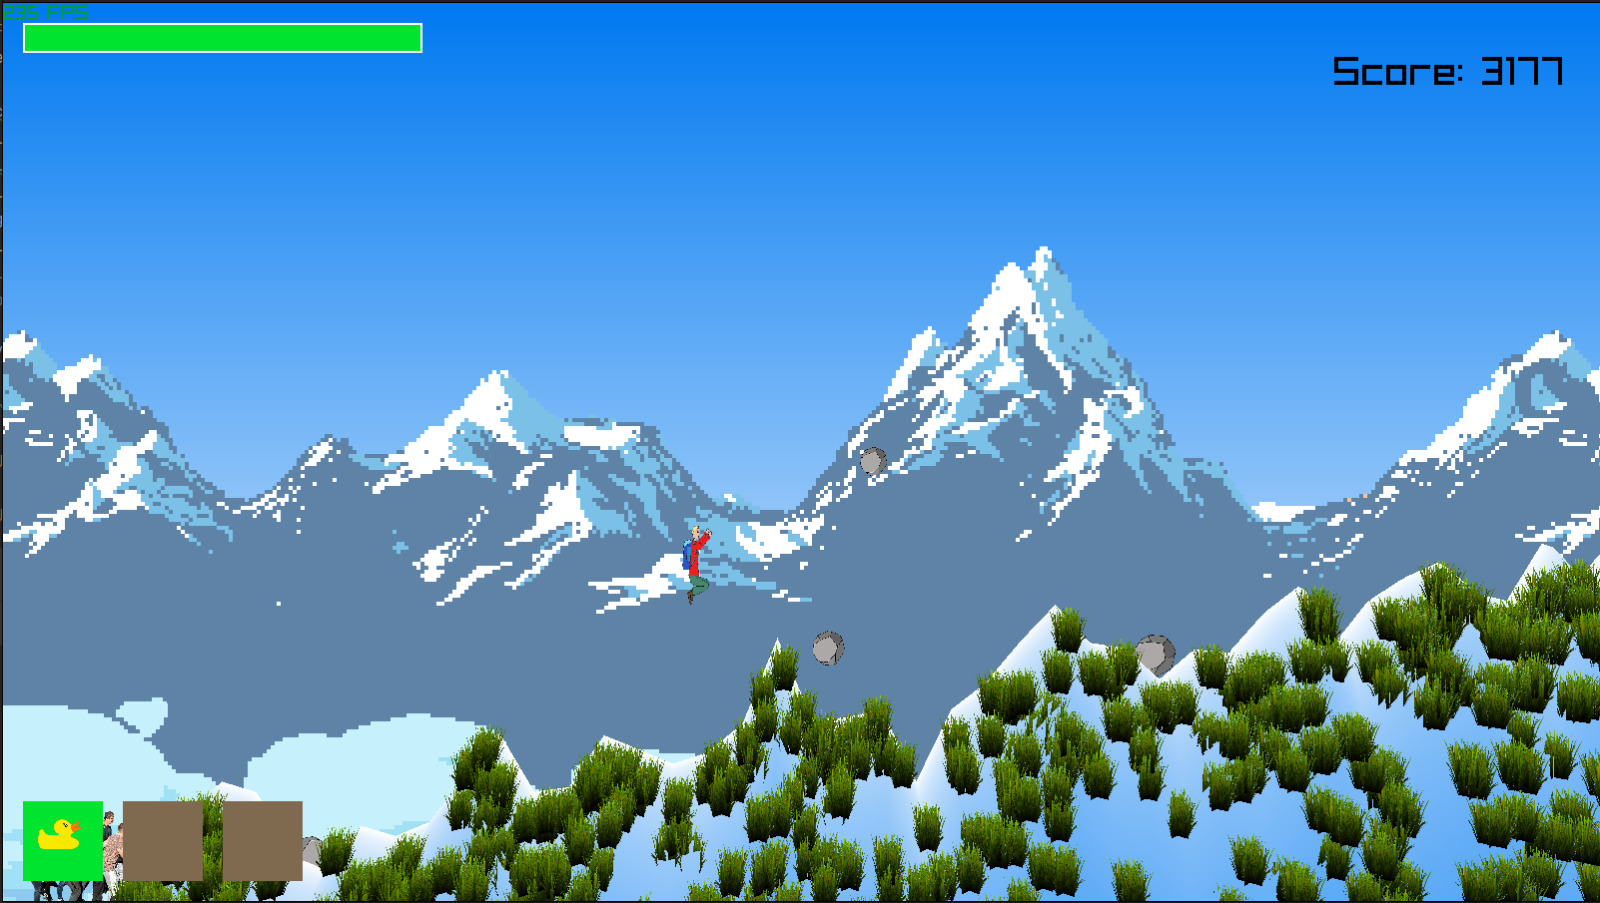
\includegraphics[width=\textwidth]{../figures/old_game.jpeg}
                    \caption{Ferienakademie 2023\phantom{y}}
                \end{figure}
            }
        \end{minipage}
        \begin{minipage}{.495\textwidth}
            \onslide<2>{
                \begin{figure}
                    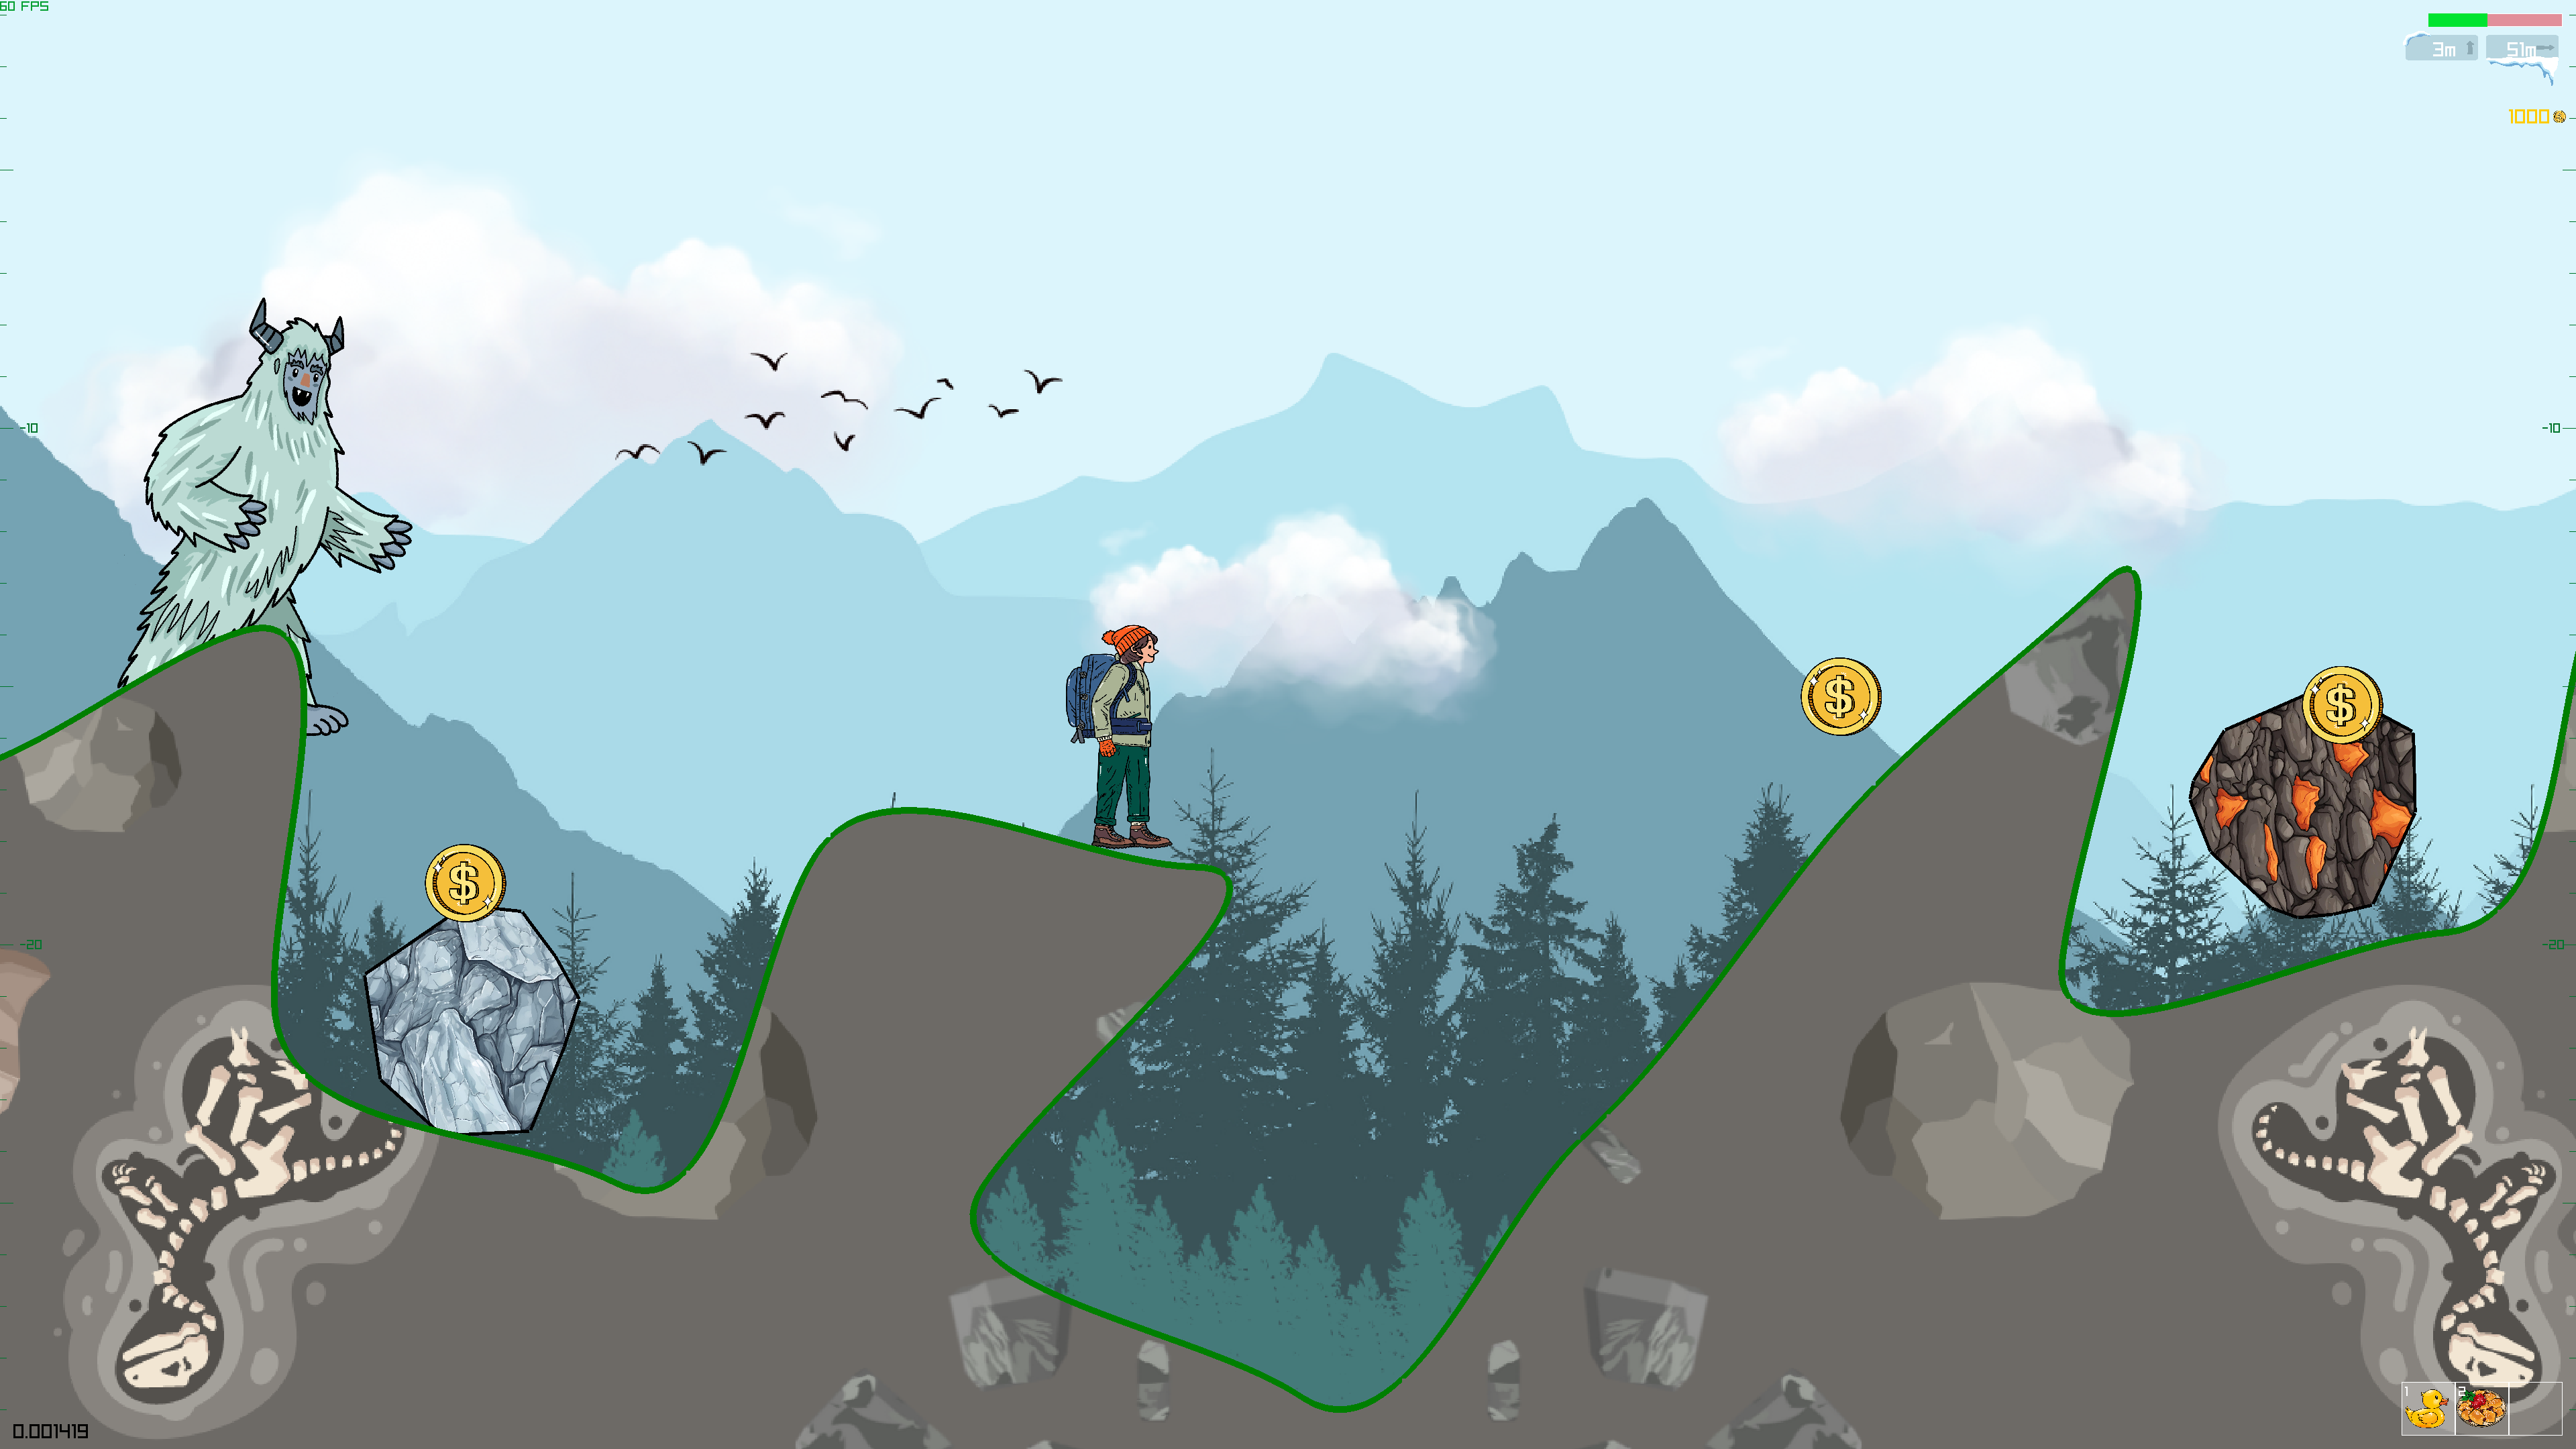
\includegraphics[width=\textwidth]{../figures/new_game.png}
                    \caption{Today}
                \end{figure}
            }
        \end{minipage}
    \end{minipage}
    %\vspace{-.45cm}
\end{frame}

\begin{frame}{A New Game with an Old Soul}
    \centering
    \begin{tabular}{cc}
        \begin{tcolorbox}[colback=boxcolor, width=0.5\textwidth, height=6.5cm, colframe=boxcolor, rounded corners]
            \textbf{Ferienakademie 2023}
            \begin{itemize}
                \setbeamertemplate{itemize item}{\textcolor{red}{\textbf{-}}}
                \item not all items have a functionality
                \item ``buggy'' physics, dependent on fps
                \item linear terrain
                \item based on Entity-Component-System
                \item[\textcolor{green}{\textbf{+}}] good performance
                \item[\textcolor{green}{\textbf{+}}] great ideas!
            \end{itemize}
        \end{tcolorbox}
        &
        \begin{tcolorbox}[colback=boxcolor, width=0.5\textwidth, height=6.5cm, colframe=boxcolor, rounded corners]
            \textbf{New "Surviving Sarntal"}
            \begin{itemize}
                \setbeamertemplate{itemize item}{\textcolor{green}{\textbf{+}}}
                \item unique items
                \item accurate physics, independent of fps
                \item spline-based terrain with overhangs
                \item increasing difficulty
                \item new audio and visuals 
                \item modular and maintainable code based on OOP
                \item addition of game menu
            \end{itemize}
        \end{tcolorbox}
    \end{tabular}
\end{frame}


\begin{frame}{Outline}
    \tableofcontents
\end{frame}


\begin{frame}{Introduction}
    \begin{itemize}
        \item Project objective: Enhance "Surviving Sarntal" with modular code, real-time physics, and improved user experience.
    \end{itemize}
    \centering
    \begin{figure}
        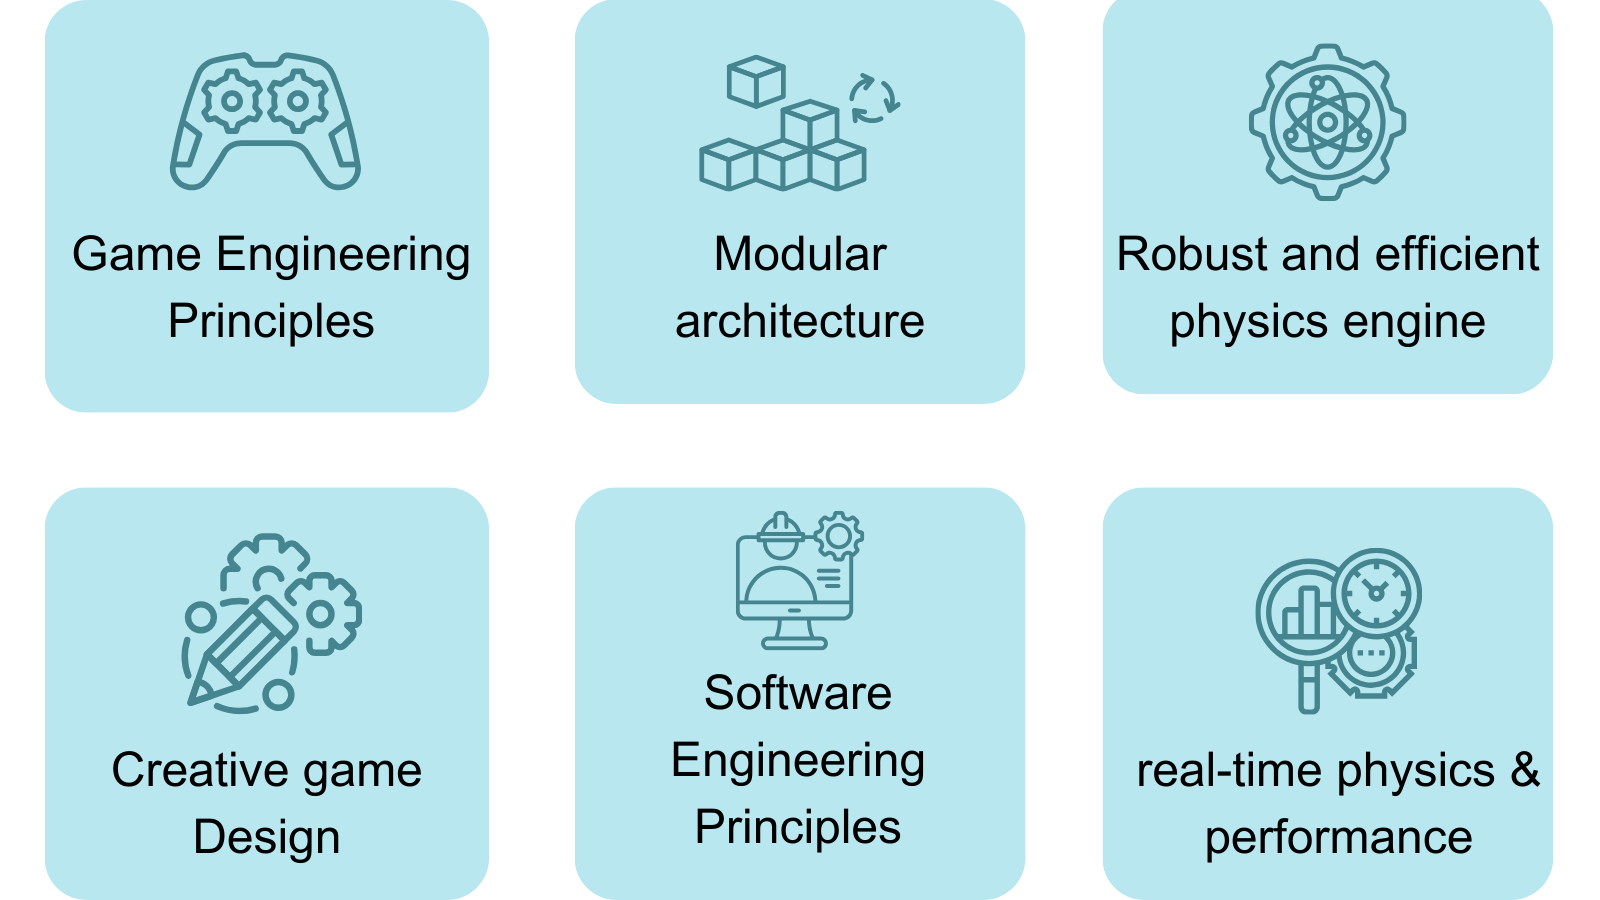
\includegraphics[width=0.65\textwidth]{../figures/focusPoints.png}
    \end{figure}
\end{frame}